\documentclass{dhbenelux}

\usepackage{booktabs} % for toprule, midrule, bottomrule in tables
\usepackage{authblk} % for multiple authors and affiliations
\usepackage{graphicx} % to inlcude graphics with \includegraphics
\usepackage{amssymb}
\usepackage{tipa}

%\DeclareUnicodeCharacter{2265}{}

\author{Megan Bushnell}

\affil{University of Oxford}

\title{Reconstructing Gavin Douglas’s Translation Practice in the \emph{Eneados} Using a Corpus Linguistic-Based Method}

\begin{document}

\maketitle
% include copright statement on first page:
\thispagestyle{papertitlepage} 

\section{Introduction}

One of the main questions in the study of translation is whether
something can be translated perfectly. Is a flawless transposition of
ideas, style, and context possible across languages? The generally
accepted answer to this question is `no'---the semantic networks of one
language are too complex to be reproduced perfectly by another. However,
closer examination of the topic reveals the issue is even more fraught,
raising questions such as how a perfect translation is defined, how to
evaluate it, and if it is even desirable. Different answers to these
questions yield different approaches to translation and different
implications as to the nature of meaning and how it is accessed. Some
approaches separate meaning from language or from its physical context.
Others, like the one pursued here, argue that meaning is
multidimensional, created not just by language, but by context and
presentation. Therefore, a multidimensional, interdisciplinary method
must be adopted when studying translation.

This paper discusses the practical application of such an
interdisciplinary method that applies digital tools and resources to the
study of medieval translation---specifically Gavin Douglas's medieval
Scottish translation of the \emph{Aeneid}, the \emph{Eneados} (1513).
This is the subject of the author's DPhil project at the University of
Oxford, titled \emph{Equivalency, Page Design, and Corpus Linguistics:
An Interdisciplinary Approach to Gavin Douglas's `Eneados'} (completed
May \citeyear{bushnell2021}), which argues that such a method can be indispensable for the
study of medieval texts by making larger texts more accessible and
offering new perspectives on them. This paper considers a specific study
directly from this doctoral work that cross references the evolution of
Douglas's translation method with changes in his source's layout. Such a
comparison reveals a new perspective on Douglas that is relevant to
longstanding critical debates on the nature of Douglas's humanism.

This paper first introduces Gavin Douglas and the \emph{Eneados} and
various critical debates regarding his translation method and humanist
status. It then discusses the interdisciplinary method adopted here that
makes use of a digital resource, designed with reference to descriptive
translation studies, corpus linguistics, and philology. This resource is
described in detail. A case study is then presented that statistically
analyses Douglas's translation method by means of line ratios---a
measure of how many lines Douglas uses to translate one line of
Latin---and compares these results to aspects of layout in Douglas's
source text. This paper evaluates these results and reflects on the
benefits and challenges of an interdisciplinary method, positing the
further potential of this method. 

\section{Gavin Douglas and the \emph{Eneados}}

The \emph{Eneados} (1513) is the first full translation of the
\emph{Aeneid} in either the English or Scottish literary tradition. It
was written by Gavin Douglas (\emph{c}. 1475-1522)---a Scottish
poet/translator, cleric, and politician, who lived on the cusp of the
Middle Ages and the emerging Renaissance, witnessing both the pinnacle
of a Scottish `golden age' under James IV and its demise (not to mention
James's) in the disastrous Battle of Flodden (1513). Consequently,
characterisations of Douglas tend to hover between oppositions---he is
either a denizen of the Middle Ages (see \citeauthor{lewis1954} 
\citeyear{lewis1954}; \citeauthor{rossi1965} \citeyear{rossi1965}; 
\citeauthor{blyth1987} \citeyear{blyth1987}) or Renaissance (see 
\citeauthor{dearing1952} \citeyear{dearing1952}; 
\citeauthor{brewerhall1960} \citeyear{brewerhall1960}; 
\citeauthor{fox1966} \citeyear{fox1966}; \citeauthor{morgan1977} 
\citeyear{morgan1977}), a vocal nationalist (see \citeauthor{canitz1996} 
\citeyear{canitz1996}; \citeauthor{corbett1999} \citeyear{corbett1999}) 
or pacifist (see \citeauthor{cummings1995} \citeyear{cummings1995}), 
and, most relevantly for this article, either a straightforward humanist 
(see \citeauthor{jack1972} \citeyear{jack1972}; \citeauthor{canitz1996} 
\citeyear{canitz1996}) or a poet to whom `a ``humanist outlook'' can only 
be ascribed ... in a highly qualified way' (\citeauthor{ross1986} 
\citeyear{ross1986}: 394).

Humanism is generally understood as `the study and imitation of
classical antiquity' (\citeauthor{wakelin2007} \citeyear{wakelin2007}: 
7). Based on the first part of this definition---the \emph{study} of 
classical antiquity involving `a self-conscious commitment to return to 
the classics' (8)---Douglas's activities definitely apply. As 
\citeauthor{jack1972} (\citeyear{jack1972}: 21) argues, `the very fact
of translating Virgil's epic indicates an interest in the humanist
ideals'. \citeauthor{johnsonpetrina2018} 
(\citeyear{johnsonpetrina2018}: x) essentially repeat this argument
when they state that the \emph{Eneados}'s purpose was `to discover the
continuity between Latin culture and its Scottish counterpart'.

However, Douglas's tendency to expand on the original text and insert
his own original poetry does not at first sight match the second
criterion---`imitation'. Throughout the thirteenth century and into the
beginning of the fourteenth, there were a series of Italian humanist
debates about the value of \emph{imitatio} with arguments over who to
imitate (several models vs. a single model, usually Cicero), what to
imitate (genre, content, or style), and what quality authors should
strive for (variety vs. consistency) (see \citeauthor{mclaughlin1996} 
\citeyear{mclaughlin1996}). Eventually (\emph{c}. 1512) this argument 
was settled by Bembo (1470-1547) in favour of single-model imitation 
valuing the replication of Cicero's style that prioritised consistency 
(see \citeauthor{mclaughlin1996} \citeyear{mclaughlin1996}: 262-74).

It is immediately apparent that Douglas does not subscribe to Bembo's
position. While Douglas's translation is notable for its extreme
fidelity to the \emph{Aeneid}, even replicating the orthography and
errors in his source---Ascensius's (\citeyear{virgil1501}) Paris 
edition of the complete works of Virgil (Ink. 4. D 7672, UB Freiburg, 
1501; see \citeauthor{bawcutt1973} \citeyear{bawcutt1973})---the 
\emph{Eneados} is also famous for its lengthy interventions in the 
original text of the \emph{Aeneid}. These include original Prologues 
to each book, as well as a thirteenth book (translated from the 
\emph{Supplement}, 1428, by Maffeo Vegio, included in Ascensius's 1501 edition), an original commentary 
(restricted to Prologue I and Book I; referred to here as the Comment),
and supplementary material throughout his translation that makes it more than twice as long
as the original (9,867 vs. 21,047 lines, excluding Book XIII and paratext). While some of this expansion
might be attributed to the fact that Douglas uses iambic pentameter,
which is a shorter line than Virgil's dactylic hexameter (see 
\citeauthor{macafee2013} \citeyear{macafee2013}: 231), much of it also 
derives from his original interpolations in the text, which consist of 
authorial asides, internal glosses, doublets and triplets, and even at 
times poetic flourishes that can make up several lines (see 
\emph{Aen}. V.429/\emph{Ene.} V.8.10-17 for a particularly extreme 
example of this). In this way, Douglas does not replicate Virgil's 
style---he does not recreate Virgil's prosody or eloquent terseness.

Douglas's humanist status is further complicated by Scotland's own
uncertain humanism during his lifetime. Printing, a key engine of
humanist activity, started late in Scotland and was initially 
sporadic, with Chepman and Myllar's press operating only briefly from 
1507-10 (see \citeauthor{dickson1885} \citeyear{dickson1885}: 9-10). 
However, despite this, or perhaps because of it, Scotland had strong 
links with the Continental book trade, which \citeauthor{ford1999} 
(\citeyear{ford1999}: 221) argues indicate strong Scottish interest 
and `participation in pressing debates of the time'---predominantly 
religious ones, but also, ostensibly, humanist. Likewise, while there 
is no discernible Greek influence (again, a hallmark of humanism) 
prevalent in Douglas's time (see \citeauthor{macqueen1990} 
\citeyear{macqueen1990}: 10), \citeauthor{jack1972} 
(\citeyear{jack1972}) observes a strong Latin and Italian humanist 
influence on Scottish authors and libraries. Indeed, Douglas himself 
proves to be highly engaged in Italian humanist authors, referencing 
them numerous times in his earlier work, the \emph{Palice of Honour} 
(\emph{c}. 1501), and proving to have intimate knowledge of some
works by Boccaccio (1313-75), Valla (1407-57), and Landino (1424-98) 
in his statements in the Prologues and Comment 
(\citeauthor{bawcutt1977} \citeyear{bawcutt1977}: 117-18).

As a result of this rather mixed humanist profile, where Douglas's
activities and context do not appear to perfectly align with humanist
sensibilities, many scholars---especially \citeauthor{gray1989} 
(\citeyear{gray1989}, \citeyear{gray2001}, \citeyear{gray2012}) have
been hesitant to outrightly classify Douglas as a humanist. Rather, 
his humanism has been qualified with such labels as `vernacular' 
(\citeauthor{bawcutt1976} \citeyear{bawcutt1976}: 36), `medieval' or 
`old' (\citeauthor{gray1989} \citeyear{gray1989}, 
\citeyear{gray2001}), `Christian' (\citeyear{gray2012}), and 
`Romantic' (\citeauthor{fowler2005} \citeyear{fowler2005}). However, 
it is this paper's contention that the confusion about Douglas's 
humanist status is rooted in his translation method, which has 
eluded comprehensive description on account of the inscrutability 
of the \emph{Eneados}.

The \emph{Eneados} is incredibly long---again, twice longer than the
original. As a result, previous studies have generally been very
selective, focusing on only one or two Books (see 
\citeauthor{blyth1987} \citeyear{blyth1987}), or just the Prologues 
(see \citeauthor{ebin1980} \citeyear{ebin1980}; 
\citeauthor{archibald1980} \citeyear{archibald1980}; 
\citeauthor{nitecki1981} \citeyear{nitecki1981}), or certain types 
of passage within the \emph{Eneados} (see \citeauthor{ridley1983} 
\citeyear{ridley1983}; \citeauthor{macafee2013} 
\citeyear{macafee2013}). While many of these selection processes are 
intelligently justified, it is hard to have a complete sense of 
Douglas's method of translation if only part of the work is analysed. 
Even those who have covered the entirety of Douglas's work (see 
\citeauthor{watt1920} \citeyear{watt1920}; \citeauthor{bawcutt1976} 
\citeyear{bawcutt1976}) have not characterised Douglas's translation 
at different points within the work, instead treating his method as 
a monolith---though Bawcutt's account is nevertheless excellent and 
a helpful critical foundation.

This paper provides a new perspective on this debate by analysing the
entirety of the \emph{Eneados} using an interdisciplinary method that
makes use of digital tools. Such a method provides a single unified
analysis of the \emph{entirety} of the \emph{Eneados} that is rooted in
both literary and quantitative analysis. The quantitative analysis
produces a `map' of the \emph{Eneados} that can make the researcher more
aware of the broader context of Douglas's work, while at the same time
providing the means to more discriminately select aspects of the texts
for literary and qualitative analysis. In the case of this study, this
method reveals an evolution in Douglas's translation method that
correlates with changes in his source text's presentation, which
indicates a greater interest in formal aspects of translation---i.e.
\emph{imitatio}---than generally granted. This, in turn, strengthens
Douglas's humanist credentials.

\section{An Interdisciplinary Method}

This project combines three subjects---descriptive translation studies
(DTS), corpus linguistics, and philology---to study Gavin Douglas's
translation of the \emph{Aeneid}. DTS is a branch of translation studies
whose aim is `to describe the phenomena of translating and
translation(s) as they manifest themselves in the world of our
experience' (\citeauthor{holmes1987} \citeyear{holmes1987}: 15). When 
identifying a work as a translation, DTS always assumes that there is a 
source text, a transferral process from the source text to the translation, 
and a tangible relationship between the translation and the original 
(\citeauthor{toury2012} \citeyear{toury2012}: 29-30). The recovery of this 
transferral process is one of the aims of DTS, and one of its main 
assumptions is that there is some form of equivalency between source- and 
target-text linguistic choices.

There are several different approaches to how this equivalency might be
understood, which might best be characterised as different permutations
of two concepts: that translation is concerned with surface-level
linguistic structures, and that translation involves the transformation
of larger cultural concepts (see \citeauthor{baker1992} 
\citeyear{baker1992}: 5-6). Modern and medieval critics have emphasised 
the importance of translation as a cultural enterprise, with modern 
scholars advising a `target-oriented approach' that focuses on the 
target-language's cultural context (see \citeauthor{vermeer1987} 
\citeyear{vermeer1987}: 29; \citeauthor{toury2012} 
\citeyear{toury2012}: 18) and medieval scholars advocating `sense for
sense' translation, as opposed to `word for word' (see 
\citeauthor{copeland1991} \citeyear{copeland1991}). Nevertheless, the 
importance of cultural context within the function of translation does 
not fully supplant its linguistic aspects. Cultural concerns dictate a 
translation's linguistic realisation, which, in turn, selects the 
appropriate translation strategies (see \citeauthor{toury2012} 
\citeyear{toury2012}: 7, fig. 2). In this way, translation processes 
and linguistic manifestations of a translation can be used to 
reverse-engineer cultural contexts.

This work attempts to do this using corpus linguistics. As 
\citeauthor{toury2012} (\citeyear{toury2012}: 243-44) notes, `it is 
precisely in the lexicon that the distinctiveness of a language 
variety used for the formulation of translations is most conspicuous'. 
Corpus linguistics provides a means of detailed analysis of a text's 
lexis by using a computer to find and count occurrences of certain 
words and analyse their contexts using statistics (see 
\citeauthor{fantinoulizanettin2015} \citeyear{fantinoulizanettin2015} 
for examples of such methods). Using this method, source texts and 
translations can be aligned to measure equivalency by means of parallel 
concordancing, where a translated text and its source can be searched 
simultaneously. This enables researchers to retrieve replacing and 
replaced segment pairs and analyse them on a large scale. Moreover, it 
enables statistical analysis, which not only helps illustrate general 
trends in the translation's process, but also indicates what aspects 
of the text deserve closer examination. In this way corpus linguistics 
can provide a different perspective on translated texts and streamline 
existing methodologies. In so doing it provides `descriptions far above 
what we live with at present' (\citeauthor{sinclair2005} 
\citeyear{sinclair2005}: 81).

However, a major flaw in the kind of description corpus linguistics
provides is that it is intrinsically divorced from its context. By its
very nature, corpus linguistics looks at language beyond its physical
form (see \citeauthor{meurman-solin2001structured} 2001: 8, 20). This can 
be a huge oversight when studying a translation---particularly a 
medieval one---as more researchers (see \citeauthor{weitemeir1996} 
\citeyear{weitemeir1996}: 101-02; \citeauthor{smithkay2011} 
\citeyear{smithkay2011}: 212; \citeauthor{kallendorf2015} 
\citeyear{kallendorf2015}: 4; \citeauthor{peikola2017} 
\citeyear{peikola2017}) acknowledge the importance of textual 
transmission in understanding a translator's reception and 
understanding of a text. This is especially vital when studying 
medieval and early modern texts, when many of the choices 
regarding book production and formatting `had not yet been standardised' 
(\citeauthor{moore2017} \citeyear{moore2017}: 23). Consequently, how a 
translation is presented can be an important consideration in how a 
translation is produced and should be factored into analysis. Such a 
practice has been labelled as `historical pragmatics' or `pragmaphilology' 
by \citeauthor{jucker1995} (1995), `philological computing' by 
\citeauthor{meurman-solin2001structured} (2001), and `historical 
pragmatics' by \citeauthor{smith2013} (\citeyear{smith2013}). The result 
is a method that is grounded in the specifics of the text, but also 
enhanced by an awareness of the text as a whole---not only in terms of a 
statistical profile of its features, but also in terms of its material 
attributes, and its historical context.

\section{The \emph{Eneados} and \emph{Aeneid} Digital Files}

To achieve this method, a collection of digital files has been assembled
using corpus linguistic methods (\citeauthor{bushnell2019gd} 2019a; 2019b). It is not strictly a corpus, as it is
made of just one text and its source material rather than
several---rather it is a `corpus-based apparatus'. It contains all
thirteen Books and Prologues of the \emph{Eneados}, along with the
twelve books of the \emph{Aeneid} and the \emph{Supplement}. It does not
contain any of the commentary included in Ascensius's (\citeyear{virgil1501}) edition, as
the transcription and digitisation of this massive commentary was beyond
the scope of this project. It comprises of 39 base files that cover
three authors (Virgil, Maffeo Vegio, and Gavin Douglas), three texts
(the \emph{Aeneid}, \emph{Supplement}, and \emph{Eneados}), and two
languages (Latin and Scots), consisting of 259,347 words total (see
Table~\ref{tab:groups}). The corpus is available online on Oxford's \emph{CQPweb}
platform (\citeauthor{hardie2012} \citeyear{hardie2012}).

\begin{table}[h]
\centering
\caption{Breakdown of the base files of the ‘corpus-based apparatus’ (\citeauthor{bushnell2019v} 2019a; 2019b).  Word counts are based on plain files—no line numbers, titles, annotation or tagging has been counted.\\}
\label{tab:groups}
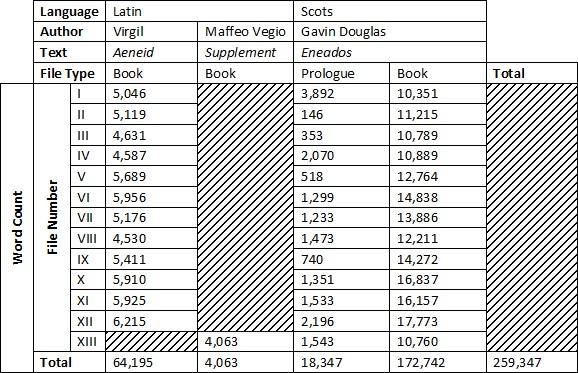
\includegraphics[width=1\linewidth]{Images/Table1.jpg}
\end{table}

\pagebreak
The digital files' sources include Coldwell's (1957-64) edition of the
\emph{Eneados} (accessed via \emph{Literature Online}) and Ascensius's
(\citeyear{virgil1501}) edition of the \emph{Aeneid}---previously established as
Douglas's source text when translating. However, Greenough's (\citeyear{virgil1897})
edition of the \emph{Aeneid} (accessed via the \emph{Perseus Digital
Library}, \citeauthor{crane1987} \emph{c}. 1987-2021) and Brinton's
(\citeyear{vegio1930}) edition of the \emph{Supplement}
(accessed via \emph{Virgil.org}, \citeauthor{wilsonokamura2014} \citeyear{wilsonokamura2014}) were also used as a base transcription
and then modified to reflect the orthography, punctuation, and content
of Ascensius's text. Coldwell's text was selected because it is the most
reliable edition of the \emph{Eneados} that is currently available,
though will soon be superseded by Bawcutt's (2020) edition, once that is
fully released. It is based on the Trinity College MS (O.3.12, Trinity
College, University of Cambridge, 1513), which is the closest to being
an exemplar out of the five extant manuscripts of the \emph{Eneados}
(Elphynstoun MS, Dk.7.49, University of Edinburgh, 1527; Ruthven MS,
Dc.1.43, University of Edinburgh, pre-1584; Lambeth MS, 117, Lambeth
Palace Library, 1545; and the Bath MS, 252A, Longleat, 1547).
Greenough's (1897-1902) and Brinton's (\citeyear{vegio1930}) texts were selected because they
were already digitised and easily accessible.

The digital files are available as plain text or as XML files. The plain
files represent the text without any metadata whatsoever. The XML files
are enhanced with several levels of metadata that describe the text's
layout, demarcate narrative and speech boundaries, and indicate
equivalent segments between the Latin and Scots. This annotation has
been implemented manually and both the Latin and Scots files are
annotated. The files are also tagged with normalised (and modernised,
where appropriate) lexical forms, and part-of-speech and semantic
labels. The normalised and modernised forms have been supplied manually,
whereas the part-of-speech and semantic tagging was provided by the USAS
tagger (see \citeauthor{archer2003} \citeyear{archer2003}). This tagging is only provided for the Scots files.

The metadata most relevant for this specific case study is the layout
and alignment annotation. Three types of layout are represented in these
files: Douglas's \emph{ordinatio} (how he breaks up his text into
chapters and books), Ascensius's \emph{ordinatio} (how he breaks up his
text into sections and books), and page divisions in Ascensius's
edition. The page breaks in the Trinity MS---widely accepted being
closest to an exemplar out of available manuscripts of the
\emph{Eneados}---are not represented, because while the number of lines
on each page in Ascensius's (\citeyear{virgil1501}) edition differs wildly over the course of
the text, it is more constant in the Trinity manuscript, where
approximately 40 lines appear on every page. As previously intimated,
Ascensius divides the \emph{Aeneid} into smaller chunks, which, at least
initially, are confined by the page, making page breaks analogous to
section boundaries. However, page breaks in the Trinity manuscript carry
no such weight. Moreover, page breaks and page layout in general in the
Trinity manuscript was probably at the discretion of Matthew Geddes, the
scribe of the Trinity MS and Douglas's secretary, rather than Douglas
himself. Ascensius's page layout, on the other hand, is original to him,
as he was the compiler of his edition and printed it in partnership with
Thielman Kerver and Jean Petit.

Alignment annotation was implemented by breaking the \emph{Aeneid} and
\emph{Eneados} into translation units. A translation unit here is
defined as whole lines (barring interference from layout) of the source
and translation that correspond to one another so that the source is
completely translated, and the translation is completely accounted for,
and that cannot be broken down into smaller units of complete
translation that also are contained within whole lines (barring
interference from layout). The following would be considered a
translation unit where one line of Latin is completely translated by
four lines of Scots:

\pagebreak
\enlargethispage{\baselineskip}
\begin{quote}
Tum decuit cum scaeptra dabas: en dextra fidesque (\citeauthor{virgil1501} \citeyear{virgil1501}: IV.597)\\

`... Sa til haue done than had bene mair ganand\\
Quhen thou hym gave the ceptour of thi land.\\
Ha! now behald hys gret prowes', quod sche,\\
`Hys reuthful piete and faith! Is not (y)on\footnote{A 'y' in parentheses signifies a yogh.} he ... ' (\citeauthor{douglas1957} 1957-64:
IV.11.23-26)
\end{quote}

The texts were aligned by line since they are both poems and their lines
are distinct units of expression. While, as noted previously, the lines
in the \emph{Aeneid} and \emph{Eneados} are of different lengths, they
at least have a functional equivalency between the two poems, are at
stable lengths, and are established components within poetry. These
factors make them the best units of measurement. However, it must be
remembered that neither Douglas nor Virgil necessarily composed using
lines as a unit of meaning.

\section{The Impact of Ascensius’s (1501) Edition on Douglas’s Evolving Translation Method}

As previously explained, Douglas's translation method has eluded
comprehensive description. This is partly because of how critics have
approached the \emph{Eneados}, but also because of the seemingly
contradictory nature of Douglas's translation. Douglas appears to
'"tie ... himself"' to the original to such an extent `as to
lose his artistic freedom' (\citeauthor{petrina2013} \citeyear{petrina2013}: 24), yet at the same time
seems perfectly untroubled exercising his poetic license regardless.
Even his conception of his practice is contradictory. In Prologue I,
Douglas makes clear that he does not pursue `word for word'---ostensibly
literal---translation, making entreaties like `I pray (y)ou note me nocht
at euery word' (\citeauthor{douglas1957} 1957-64: I.Prol.126). However, he later declares in his Direction (ll. 44-46)---a postscript addressed to his patron---that readers can compare
his translation to its source and account for almost every word.

Fortunately, the process of aligning digital files of the \emph{Aeneid}
and \emph{Eneados} has created a means of measuring the distance between
the original text and translation via line ratios---the measure of how
many lines Douglas uses to translate one line of Latin. These
effectively measure how closely Douglas mimics surface level structures
in the original Latin text---specifically the length of clauses. Out of
the 6,311 translation units in the \emph{Eneados}, 54\% have a line
ratio with the value of 2 (\emph{p} \textless{} 0.001, pairwise
proportion test), with usually 1
line of Latin being translated with 2 lines of Scots (70\%, \emph{p}
\textless{} 0.001, pairwise proportion test). This confirms Bawcutt's (\citeyear{bawcutt1974}: 57) claim that, for Douglas,
`the couplet often corresponds to a single hexameter' and suggests that
Douglas translated line by line.

Such practice is conducive for literal translation---understood here as
a translation that follows the syntax of its source very closely---as it
forces the translator to maintain the order of content in the poem and
encourages the preservation of the original grammar, whereas larger
translation units enable a less meticulous approach to translation (i.e.
paraphrase). For example, the following translation unit features a line
ratio of 1.88, which does not indicate an especially expansive
translation. However, the unit itself is very large (15:8) indicating
that rather than translate this instance line by line, Douglas decided
to translate part of Aeneas's defence when reproached by Dido as a
block. While this is not an inappropriate decision, considering that
these lines feature several incidents of enjambment, suggesting that
they are meant to be read together, this is an unusual decision for
Douglas, who structures his translation around single lines of Latin
56\% of the time (\emph{p} \textless{} 0.001, pairwise proportion test),
even though Virgil's lines are not always designed to stand alone in this way.

\begin{quote}
Pro re pauca loquar: nec ego hanc abscondere furto\\
Speraui: ne finge fugam: nec coniugis vnquam\\
Praetendi tedas: aut haec in foedera veni.\\
Me si fata meis paterentur ducere vitam\\
Auspiciis: et sponte mea componere curas\\
Vrbem troianam primum dulcesque meorum\\
Relliquias colerem: et priami tecta alta manerent.\\
Et recidiua manu posuissem pergama victis: (\citeauthor{virgil1501} \citeyear{virgil1501}: IV.337-44)\\

'... As the mater requiris, a litil heris:\\
I purposyt nocht forto hyde thyftuusly\\
My vayage, nor, as (y)e weyn, secretly\\
Away to steil; quhat nedis (y)ou sa tofeyn?\\
For I pretendit nevir, be na meyn,\\
With (y)ou to mak the band of mariage,\\
Nor in that (y)ok, ne frendschip in Cartage,\\
(Y)yt come I nevir: bot gif the fatis, but pled,\\
At my plesour sufferit me lyfe to led,\\
At my fre wil my warkis to modyfy,\\
The cite of Troy than first agane suld I\\
Restore, and of our deir frendis remanys\\
Gaddir togiddir, and to the venquist Troianys\\
Raparal with my handis agane thar wallis,\\
And beild vp Priamus palyce at now fallis. ...' (\citeauthor{douglas1957} 1957-64:
IV.6.112-26)
\end{quote}

In not approaching this passage line by line, Douglas can play with the
order of things and does not adhere as closely to the syntax of the
passage. Every Latin line in this passage is interspersed with another
within the Scots translation---except for the last two lines
(\emph{Aen.} IV.343-44, \emph{Ene.} IV.6.125-26), which are completely
swapped in their order of translation. There is also some paraphrase and
doubling that accompanies this rearrangement. For example, Douglas
translates `abscondere' (`to abscond') twice two lines apart as `forto
hyde thyftuusly' (\emph{Ene.} IV.6.113) and `away to steil' (IV.6.115).
Likewise, he paraphrases `ne finge' (`do not pretend') twice in separate
lines---once as `as {\textyogh}e weyn'
%lines---once as `as ȝe weyn'
(IV.6.14) and again as `quaht nedis {\textyogh}ou sa
%(IV.6.14) and again as `quaht nedis ȝou sa
tofeyn' (IV.6.15). He also arguably translates `componere' (`to put in
order, to gather together') and `colerem' (`I would take care of')
twice. Both are translated initially as `my warkis to modyfy' and `The
cite of Troy ... suld I / Restore'. However, then Douglas appears to
combine the meaning of `componere' with the subjunctive force of
`colerem' when he has Aeneas declare `suld I ... of our deir frendis
remanys / Gaddir togiddir'. He similarly blurs his translations of
`posuissem' (`I would establish') and `manerent' (`they would endure').
Not only does he take `manerent' as a first person singular form, when
it is really third person plural, but his translation `beild vp' is
arguably more appropriate for `posuissem', since it suggests the
creation of something new, whereas `reparal', the translation for
`posuissem', implies the restoration of something old. In effect,
Douglas takes a case of \emph{dicolon abundans}---a rhetorical trope
where Virgil repeats the same idea in a different manner (see \citeauthor{dainotti2015} \citeyear{dainotti2015}: 35)---and shares vocabulary between the two Latin
iterations. He is enabled to do so by translating a larger section of
Latin at one time, as this gives him more options for translation. He
can decide what content should go together and how the grammar should be
interpreted. As result, the syntax of the passage is more loosely
rendered.

\pagebreak
By contrast, a smaller translation unit produces a far more exact
translation. The following example, featuring the Sibyl's instructions
to the Trojans, has a high line ratio of 4 (4:1), but the unit itself is
small, indicating how Douglas was translating this passage line by line
(see \emph{Aen.} VI.125-55/\emph{Ene.} VI.2.100-57; average line ratio:
2.9; average number of Latin lines per unit: 1.5).

\begin{quote}
Duc nigras pecudes: ea prima piacula sunto: (\citeauthor{virgil1501} \citeyear{virgil1501}: VI.153)\\

Til his funeral entyre, or sacrifyss,\\
Do bring the blak bestis, as is the gyss;\\
Lat tha be {\textyogh}our first expiationys,\\
And clenging graith, eftir {\textyogh}our serymonys. (\citeauthor{douglas1957} 
%Lat tha be ȝour first expiationys,\\
%And clenging graith, eftir ȝour serymonys. (\citeauthor{douglas1957} 1957-64:
VI.2.151-54)
\end{quote}

While this unit features many additions that serve to clarify Sibyl's
orders, the translation is grammatically exact so that the imperative
verbs `duc' (`bring') and `sunto' (`let be') are translated literally.
Such translation proves to be the norm for Douglas, as corroborated by a
qualitative analysis of Douglas's most expansive (where line ratios are
4 or greater) and succinct (where line ratios are 1 or less) translation
units (see Figure~\ref{fig:figure1} for a summary of results).

\begin{figure}[H]
% Use center to align a figure or table to the middle of the text column
\begin{center}
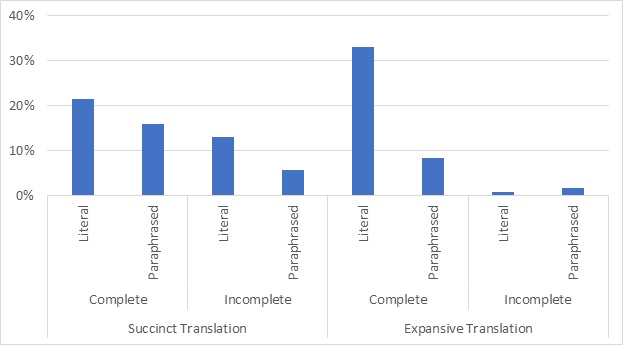
\includegraphics[width=1\linewidth]{Images/Figure1.jpg}
\end{center}
\caption{Distribution of four different combinations of literal, paraphrased, complete, and incomplete translation across translation units that have very low (less than or equal to 1) or high (greater than or equal to 4) line ratios.  Results are significant according to a chi-square test (\emph{p} < 0.001).}
\label{fig:figure1}
\end{figure}

However, while this preference for lengthy, literal translation often
characterises Douglas's method, the implementation of `standard' line
ratios and units (where 2 lines of Scots translate 1 line of Latin) is
irregular and uneven. A closer look at the line ratios in the
\emph{Eneados} reveals a general increase in Douglas's length of
translation over the course of the \emph{Eneados} (Figure~\ref{fig:figure2}). This
expansion is only partly based off Virgil's own tendencies. While Virgil
also becomes more expansive throughout the \emph{Aeneid}, writing longer
and longer books, the change is less dramatic (Figure~\ref{fig:figure3}). The
\emph{Eneados} adds about 59 extra lines per book, while the
\emph{Aeneid} adds only 6---in other words, Douglas is almost ten times
more prolific than Virgil.

\begin{figure}[H]
% Use center to align a figure or table to the middle of the text column
\begin{center}
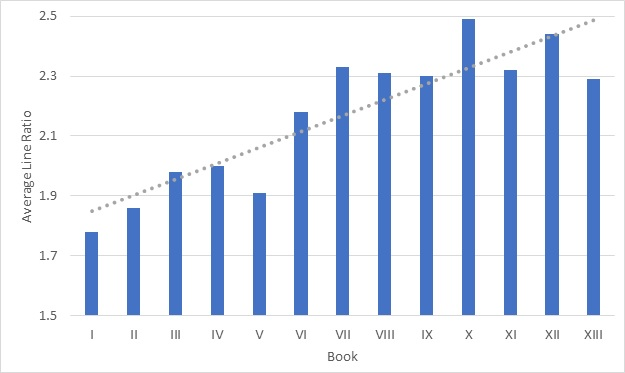
\includegraphics[width=1\linewidth]{Images/Figure2.jpg}
\end{center}
\caption{Average line ratios across the thirteen books of the \emph{Eneados} with a descriptive trend line.  Results are significant (\emph{p} < 0.001) according to a linear regression performed in R that was tested with an ANOVA.}
\label{fig:figure2}
\end{figure}

\begin{figure}[H]
% Use center to align a figure or table to the middle of the text column
\begin{center}
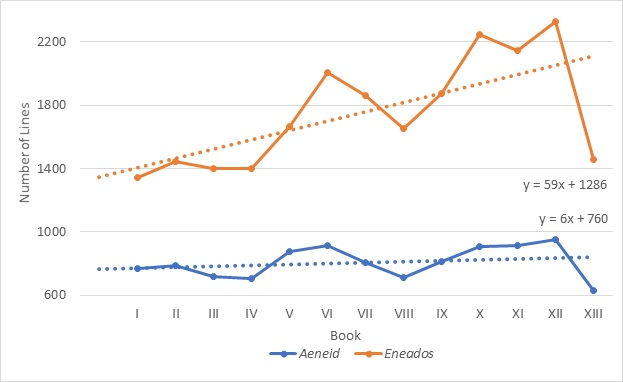
\includegraphics[width=1\linewidth]{Images/Figure3.jpg}
\end{center}
\caption{Total number of lines in each book of the \emph{Aeneid} and \emph{Eneados} with linear trend lines and equations.  The results are significantly different (\emph{p} < 0.001) according to a t-test.}
\label{fig:figure3}
\end{figure}

\pagebreak
\begin{figure}[H]
% Use center to align a figure or table to the middle of the text column
\begin{center}
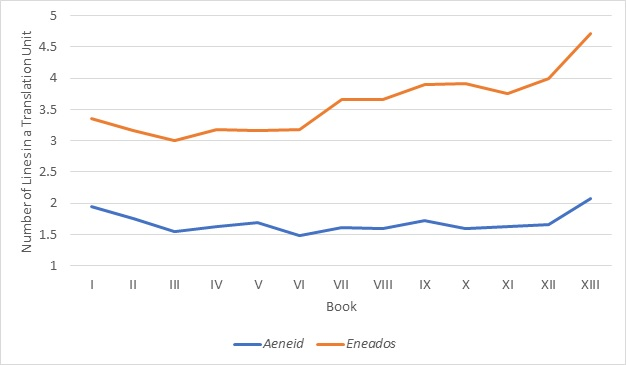
\includegraphics[width=1\linewidth]{Images/Figure4.jpg}
\end{center}
\caption{Average number of Latin and Scots lines in every translation unit in every book of the \emph{Eneados}.  Results are significant for both Latin and Scots data (\emph{p} < 0.001) according to a linear regression performed in R that was tested with an ANOVA.}
\label{fig:figure4}
\end{figure}

Not only do Douglas's line ratios change over the course of the
\emph{Eneados}, but the number of Latin and Scots lines per unit changes
too (Figure~\ref{fig:figure4}). For the most part, the number of Latin lines in each
translation unit remains constant around 1.5, indicating that Douglas
generally translates on a line by line basis. However, in Book I and
Book XIII the number spikes to 2, which could indicate an increase in
paraphrased translation, as in the example below from Book I where Douglas
paraphrases `olim voluentibus annis' (`at long last after years have
turned') as `efter this mony a day', `reuocato a sanguine teucri'
(`recalled from the blood of Teucer') as `of Troianys ofspring', and
combines `ductores' (`princes'), `qui mare: qui terras omni ditione
tenerent' (`who hold the sea, who hold lands with sovereignty') as
`princis of power our sey and land to ryng'.

\begin{quote}
`... Cunctus ob italiam terrarum clauditur orbis.\\
Certe hinc romanos olim voluentibus annis\\
Hinc fore ductores: reuocato a sanguine teucri:\\
Qui mare: qui terras omni ditione tenerent\\
Pollicitus: quae te genitor sententia vertit? ...' (\citeauthor{virgil1501} \citeyear{virgil1501}:
I.233-37)\\

`... Throu owt the warld debarrit in euery sted\\
And drevin from Itale? Thou hecht vmquhill, perfay,\\
Of thame suld cum, efter this mony a day,\\
The worthy Romanys, and of Troianys ofspring\\
Princis of power our sey and land to ryng.\\
Quhat wikkit counsale, fader, has turnyt thi thocht? ...' (\citeauthor{douglas1957} 1957-64: I.5.16-21)
\end{quote}

This less syntactically exact translation might be expected for Book
XIII, given that Book XIII draws on the work of a different author
\citep{virgil1501} and Douglas's respect for this work
is significantly less than that for the \emph{Aeneid} (see \citeauthor{ghosh1995} \citeyear{ghosh1995}:
7). However, it is surprising that Douglas should have adopted a similar
approach to Book I, when he praises Virgil so highly in Prologue I. This
suggests that Douglas begins translating the \emph{Aeneid} in one
fashion, but then chooses to pursue a more grammatically exacting one
for the rest of the poem. He resurrects this more flexible model only in
Book XIII---either because he has less respect for Vegio as a poet or
because aspects of Vegio's text necessitate it. This indicates a general
push towards literal translation over the course of the \emph{Eneados},
confirmed by Figure~\ref{fig:figure5}.

\begin{figure}[H]
% Use center to align a figure or table to the middle of the text column
\begin{center}
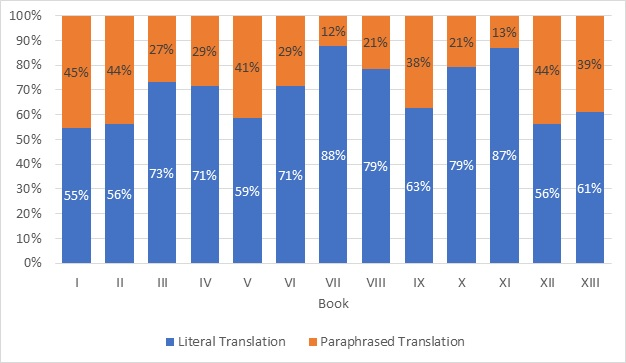
\includegraphics[width=1\linewidth]{Images/Figure5.jpg}
\end{center}
\caption{Distribution of literal and paraphrased translation in selected translation units with very low (less than or equal to 1) or high (less than or equal to 4) line ratios in each book of the \emph{Eneados}.  Results are significant according to a chi-square test (\emph{p} < 0.01).}
\label{fig:figure5}
\end{figure}

Such variation in activity indicates that Douglas's translation practice
evolves, which would mean that translation is not a uniform action even
when performed by a single translator for a single text. This would also
imply that Douglas translates the \emph{Aeneid} in its textual order.
This makes sense, given that translation is essentially a product of
reading, and thus dictated by the source text's \emph{ordinatio}. In
fact, this increase in Douglas's line ratios over the course of the
\emph{Eneados} can be attributed to the evolution in the layout of his
source text---Ascensius's (\citeyear{virgil1501}) edition.

The layout of Ascensius's (\citeyear{virgil1501}) text is somewhat complex. Excerpts from the
\emph{Aeneid} are foregrounded in the page and surrounded by two
accompanying commentaries---one by Servius and one by himself (Figure~\ref{fig:figure6}). While this was a common way of presenting the text in printed
editions of the \emph{Aeneid} of this time, Ascensius's segmentation of
the text is unique in that he endeavours to ensure that his excerpts
make grammatical or narrative sense, whereas other editions tend to
follow segmentation that is dictated by the commentary rather than the
text. In fact, a comparison of the segmentation in Ascensius's edition
to that in six other texts (\citeauthor{virgil1487} 1487/88; \citeauthor{virgil1491} 1491-92; \citeauthor{virgil1492antonius} 1492a; \citeauthor{virgil1492liga} 1492b; \citeauthor{virgil1492anton} 1492c; \citeauthor{virgil1499} 1499) reveals
only a 9\% similarity, whereas the other editions have, on average, a
97\% similarity between each other (\emph{p} \textless{} 0.001, pairwise
proportion test).

\begin{figure}[H]
% Use center to align a figure or table to the middle of the text column
\begin{center}
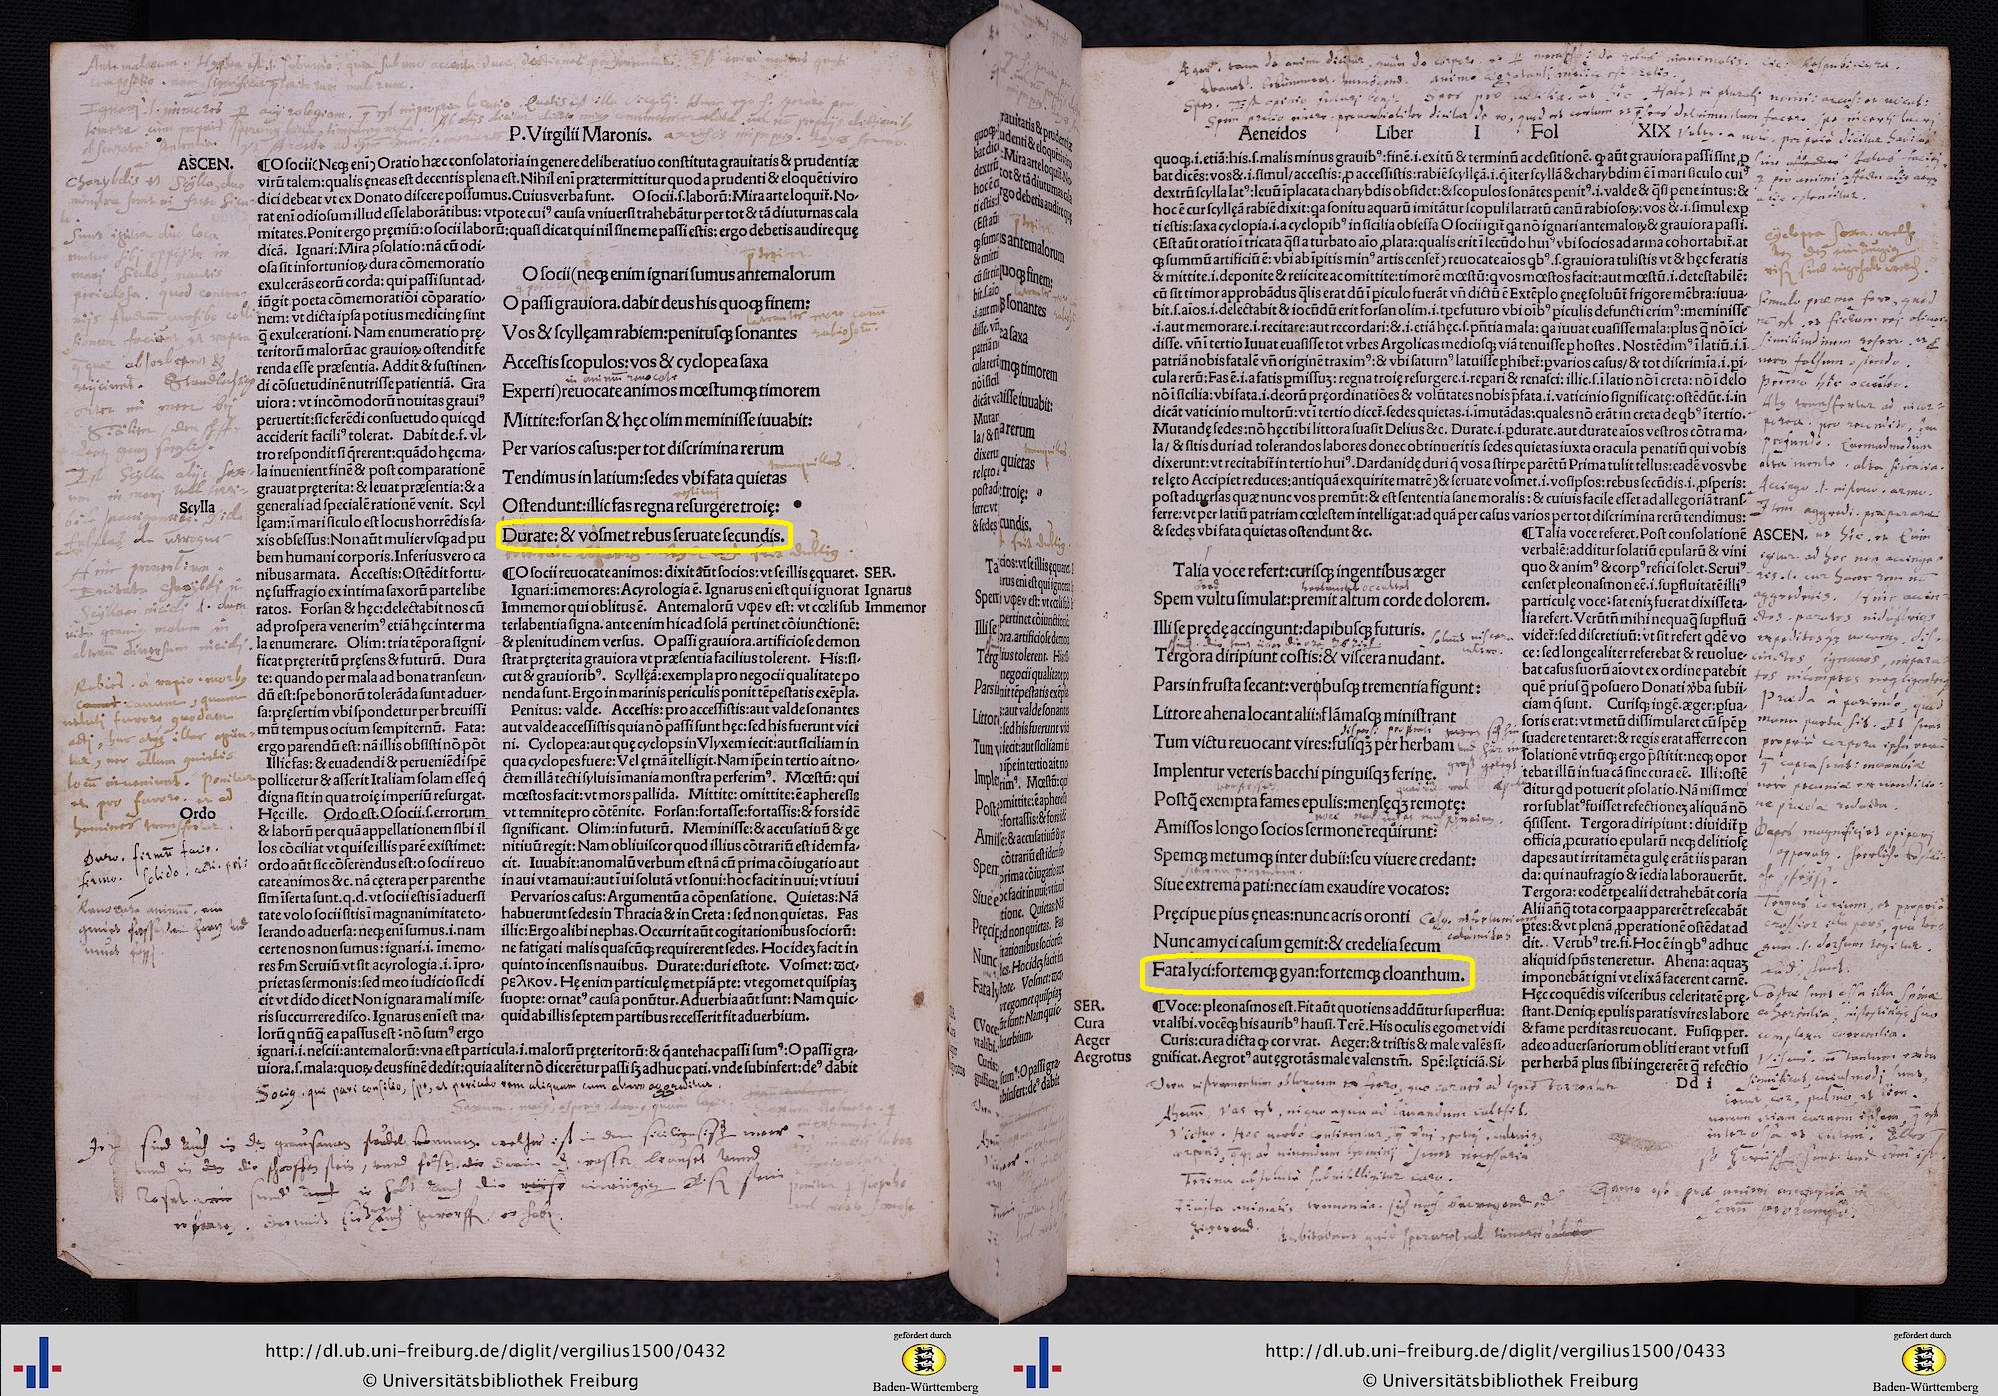
\includegraphics[width=1\linewidth]{Images/Figure6.jpg}
\end{center}
\caption{UB Freiburg, Ink. 4. D 7672 fol. 18v-19r, featuring \emph{Aen}. I.198-222; image has been cropped.  This is a typical layout in Ascensius’s edition for the early books.  Lines \emph{Aen}. I.207-08 are highlighted (my edit) to illustrate an example below.}
\label{fig:figure6}
\end{figure}

Douglas proves to be sensitive to this aspect Ascensius's layout,
structuring his chapters around Ascensius's sections 67\% of the time
(\emph{p} \textless{} 0.001, pairwise proportion test), with two sections on average comprising a chapter---as
Bawcutt (1976: 105) estimates. For example, the following chapter break
imitates the section break in Figure~\ref{fig:figure7}.

\begin{quote}
... hunc claris dextera factis.\\
{[}Section break here.{]}\\
Dum turnus rutulos animis audacibus implet. (\citeauthor{virgil1501} \citeyear{virgil1501}: VII.474-75)\\

... And sum war eik inducit to the weir\\
For hie prowes knawin in ilke landis,\\
And dedis wrocht maste knychtly with his handis.\\

{[}Chapter break here.{]}\\
Ascanyus huntand hass a taym hart hurt,\\
Quhilk was the first moving of strife and sturt.\\

Quhill Turnus on this wyss, about all partis,\\
In the Rutilyanys rasys hardy hartis. (\citeauthor{douglas1957} 1957-64: VII.8.152-9.2)
\end{quote}

\begin{figure}[H]
% Use center to align a figure or table to the middle of the text column
\begin{center}
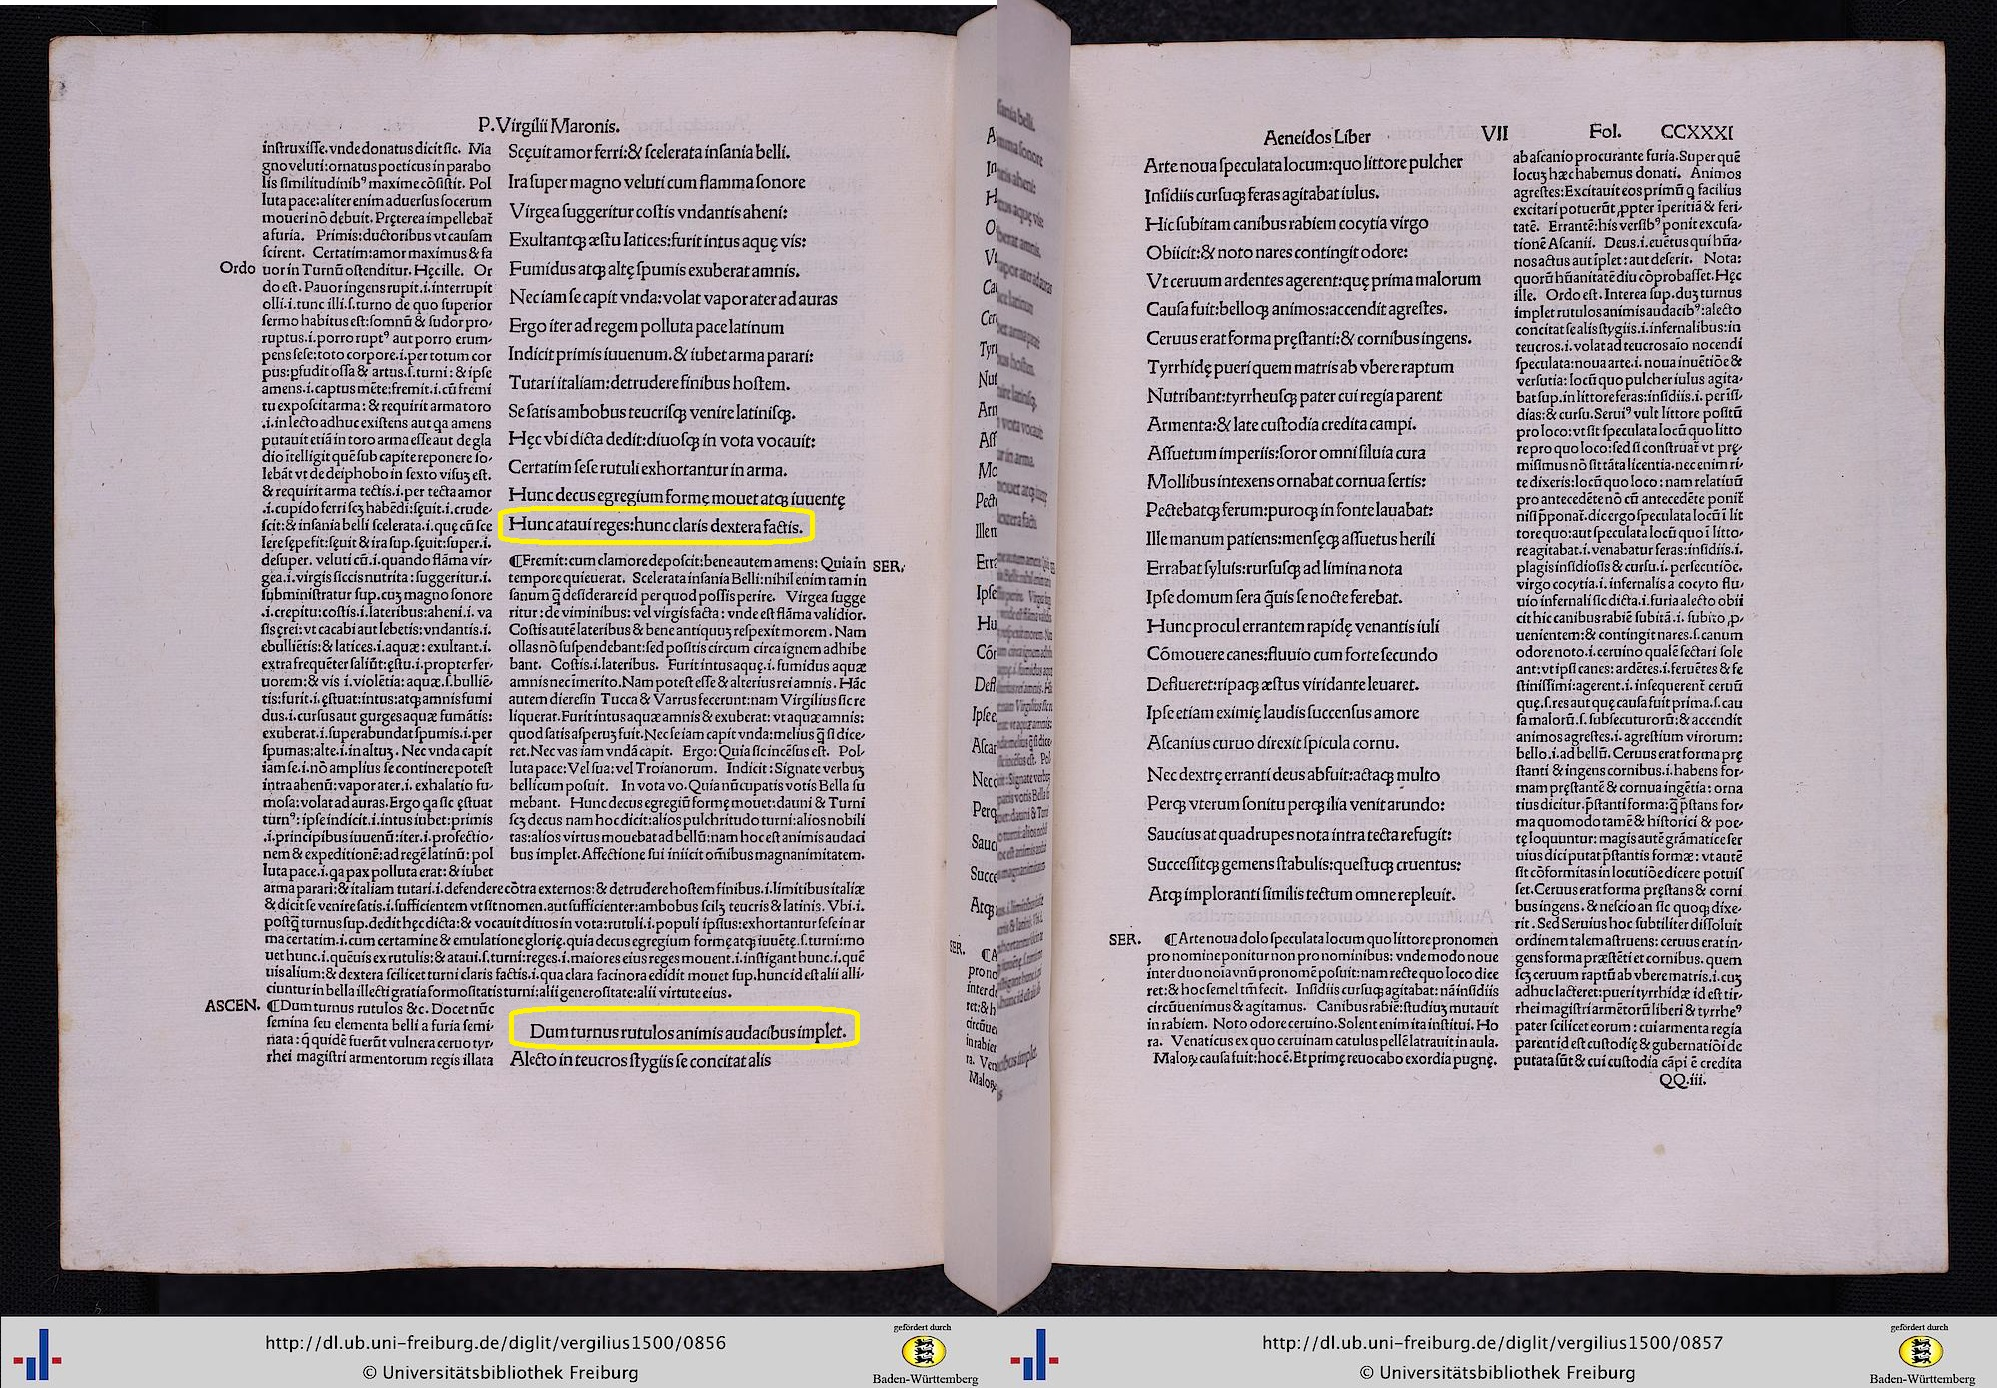
\includegraphics[width=1\linewidth]{Images/Figure7.jpg}
\end{center}
\caption{UB Freiburg Ink. 4. D 7672 Folio 230v-231r in, featuring \emph{Aen}. VII.461-502; image has been cropped.  Lines \emph{Aen}. VII.474-75 are highlighted (my edit) to illustrate the example above.}
\label{fig:figure7}
\end{figure}

Similarly, 99.5\% of the time (\emph{p} \textless{} 0.001, pairwise
proportion test), Douglas honours these sections
within his translation units. For example, the following translation
units (labelled with large brackets) preserve the section break seen in
Figure~\ref{fig:figure6}:

\begin{quote}
Durate: et vosmet rebus seruate secundis. (\citeauthor{virgil1501} \citeyear{virgil1501}: I.207)\\

Beis stowt on prosper forton to remane. (\citeauthor{douglas1957} 1957-64: I.4.84)\\

{[}Section break here.{]}\\

Talia voce refert: curisque ingentibus aeger ... (\citeauthor{virgil1501} \citeyear{virgil1501}: I.208)\\

Syk plesand wordis carpand he has furth brocht,\\
Set his mynd trublit mony grewouss thocht. (\citeauthor{douglas1957} 1957-64: I.4.85-86)
\end{quote}

Considering Douglas's attention to relatively minor details of
Ascensius's layout, his reaction to more noticeable aspects---such as
the dramatic transformation of layout over the course of the
text---should also be considered. In the early books, excerpts from the
\emph{Aeneid} tend to be short and rarely cross page boundaries (see
Figure~\ref{fig:figure6}). Servius's and Ascensius's commentaries, on the other hand,
are very lengthy and frequently spill over the page. In the later books
of the \emph{Aeneid}, the layout changes and the ratio of text to
commentary reverses (see Figure~\ref{fig:figure7} and Figure~\ref{fig:figure8}). This is not a sudden change but
happens gradually, starting in Book II. Excerpts from the \emph{Aeneid}
become much longer and often cross at least a single page
boundary---sometimes two. Meanwhile, the commentary shrinks.

\pagebreak
\enlargethispage{\baselineskip}
\begin{figure}[H]
% Use center to align a figure or table to the middle of the text column
\begin{center}
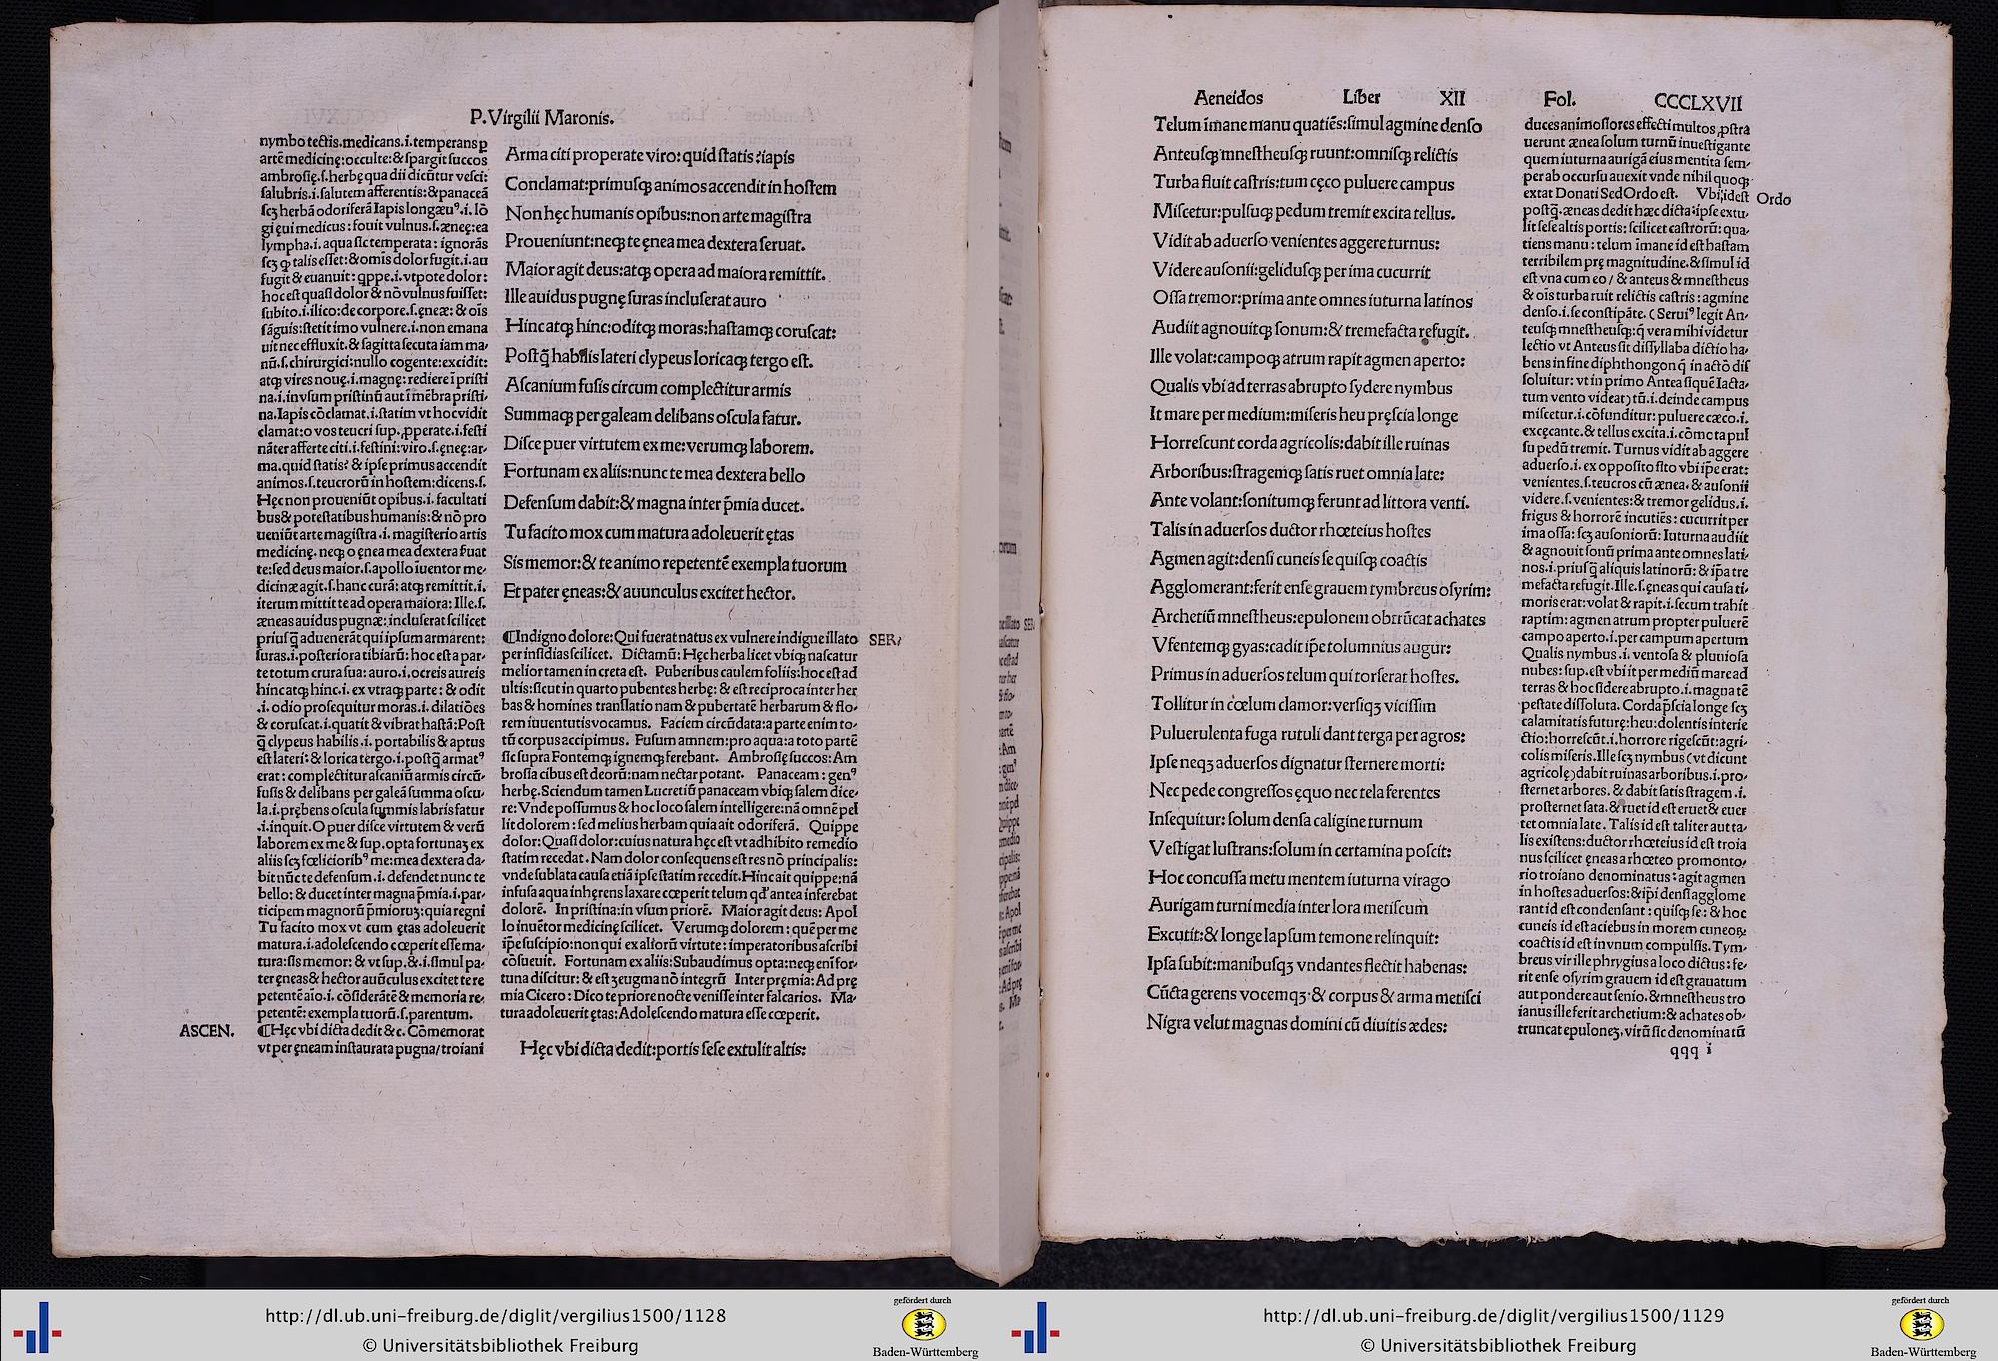
\includegraphics[width=1\linewidth]{Images/Figure8.jpg}
\end{center}
\caption{UB Freiburg, Ink. 4. D 7672 fol. 366v-367r, featuring \emph{Aen}. XII.425-73; image has been cropped.  This is a typical layout in Ascensius’s edition for the later books.}
\label{fig:figure8}
\end{figure}

This imbalance is the product of the division between the first and last
six books of the \emph{Aeneid} which has become codified in critical
traditions of Virgilian reception. `Interpretation of Books I through VI
followed the outlines established by ancient commentaries on Homer's
\emph{Odyssey}', and tended to be more weighty, whereas `Commentary on
the second half of the \emph{Aeneid} was less focused', and more sparse
(\citeauthor{wilsonokamura2010} \citeyear{wilsonokamura2010}: 191). Based on this, \citeauthor{wilsonokamura2010} (\citeyear{wilsonokamura2010}:
217), in his examination of the reception of Virgil's works in the
Renaissance, has suggested there are two different types of readers of
the \emph{Aeneid}: those who are twelve-book readers---who read the
entirety of the \emph{Aeneid} as a cohesive whole---and those who are
six-book readers---who either focus entirely on the first six books, or
who read the work as a bifurcation. It is the tradition of six-book
reading that causes the transformation of layout evident in Ascensius's
text. However, this does not necessarily mean that Ascensius himself was
a six-book reader, especially considering how he writes commentary for
the entirety of the \emph{Aeneid} and includes Maffeo Vegio's
\emph{Supplement}. It does, however, indicate that this division was a
fixture in the study of the \emph{Aeneid} at the time, resulting in more
resources being available for Books I-VI than for Books VII-XII.

It is this paper's contention that this change in layout affects the
change in Douglas's translation noted above, by means of Douglas's
interaction with Ascensius's commentary. \citeauthor{bawcutt1973} (\citeyear{bawcutt1973}: 222) observes
Douglas's original additions within the text are regularly sourced from
Ascensius's commentary. This work confirms this by examining all
translation units in the \emph{Eneados} with a line ratio greater than 4
and their available commentary resources in Ascensius's (\citeyear{virgil1501}) edition,
determining that 86\% of these units sourced their expansions directly
from Servius's and Ascensius's commentaries (\emph{p} \textless{} 0.001,
pairwise proportion test). For example, Douglas
uses both Ascensius's and Servius's commentaries when translating
Virgil's brief reference to Castor and Pollux:

\begin{quote}
Si fratrem pollux alterna morte redemit. (\citeauthor{virgil1501} \citeyear{virgil1501}: VI.121)\\

Or gif Pollux redemyt his broder Castor,\\
As he that was immortal get and boyr,\\
Partyng with him his immortalite,\\
Athir for other sufferand forto de,\\
That ych of thame, by coursis alternate,\\
Sa oft gais and returnys that gait. (\citeauthor{douglas1957} 1957-64: VI.2.87-92)
\end{quote}

The expansion `immortal get and boyr' is almost certainly from Servius's
note `Helena et pollux de ioue nati immortales fuerunt' (\citeyear{servius1501}:
fol. 176\textsuperscript{r}) or `Helen and Pollux were the immortal children
of Jupiter'. Likewise, Douglas's loose translation of `alterna morte' as
`athir for other sufferand forto de' is probably from Ascensius's note
`morte alterna id est quam alternatim pro illo obit vt ille vicissim pro
polluce' (\citeyear{ascensius1501}: fol. 176\textsuperscript{r}) or `reciprocated death, that is, how
by turns Pollux dies for the other, Castor, so that, in exchange, the
other may do the same for him'.

Similarly, Douglas mines Ascensius's and Servius's commentaries to find
synonyms for certain words. For instance, in his translation of `Et nos
et tua dexter adi pede sacra secundo' (\citeauthor{virgil1501} \citeyear{virgil1501}: VIII.302) (`come to
both us and your offerings by good speed'), \citeauthor{douglas1957} (1957-64: VIII.5.59)
translates `secundo' both as `happy' and `prosper'---the latter of which
probably comes from \citeauthor{servius1501}'s (\citeyear{servius1501}: fol. 254\textsuperscript{r}) gloss
`prospero omine' or `favourable omen'. In addition, \citeauthor{ascensius1501} (\citeyear{ascensius1501}:
fol. 254\textsuperscript{v}) glosses `adi' (`approach'), as `aggredere'
(`approach', `come here'), which matches up with \citeauthor{douglas1957}'s double
translation `wissy, at thou may cum heir' (1957-64: VIII.5.58). In this
way, Douglas uses Ascensius's text as a glossary and encyclopaedia and
incorporates it into his translation, thus impacting his textual
proportions. This, coupled with the increase in expansions throughout
the \emph{Eneados}, suggests that as Douglas translates, he relies more
and more on Ascensius.

However, this is complicated by the fact that Ascensius's commentary
decreases over the course of his edition. Rather than the amount of
commentary available, it is layout that facilitates Douglas's
expansions, as Ascensius's longer sections and shorter general
commentary in the later books allow for easier cross-referencing because
the text and the relevant commentary frequently appear on the same or
facing page. Figure~\ref{fig:figure9} shows this effect on a larger scale throughout the
\emph{Eneados}, indicating the number of sources Douglas uses and their
location in respect to the content they explain. Commentary on the
facing page of the text of the \emph{Aeneid} tends to be referenced the
most, with material that is on the same or backing page more commonly
unrecognised.

While these results are not significant (\emph{p} = 0.30, Fisher's Exact
Test, etc.), this preference is nevertheless noteworthy considering how
Ascensius presents commentary relative to each \emph{Aeneid} excerpt.
Servius's commentary always appears underneath the excerpt, while
Ascensius's own commentary runs alongside. Moreover, Ascensius's
commentary has three separate---though not always formally
distinct---parts that always appear in the same order: first, a general
summary of the excerpt (see \citeauthor{white2013} \citeyear{white2013}: 79-81), followed by quotations
by Donatus (late 4\textsuperscript{th}-early 5\textsuperscript{th} c.
AD) and sometimes Beroaldo (1453-1505) (see \citeauthor{white2013} \citeyear{white2013}: 221), ending
with a word-by-word dissection of the passage introduced by the phrase
`ordo est' (`the order is') (see \citeauthor{white2013} \citeyear{white2013}: 79-80). The two sources of
commentary Douglas uses most are Servius's commentary and Ascensius's
word-by-word dissection, which both always occur after the text they
refer to, rather than beside it, and thus rarely occur on the same page
as the text. This makes the high results for same page commentary
striking.

\begin{figure}[H]
% Use center to align a figure or table to the middle of the text column
\begin{center}
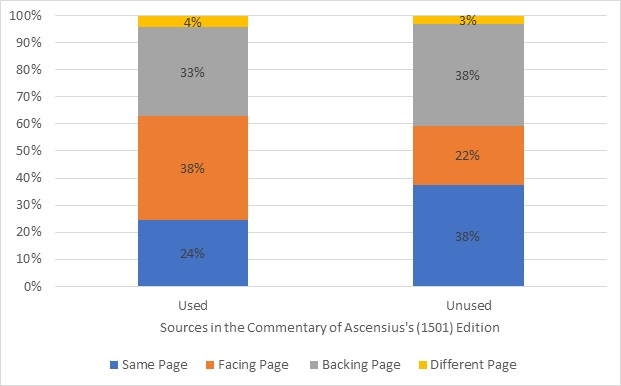
\includegraphics[width=1\linewidth]{Images/Figure9.jpg}
\end{center}
\caption{Percentage of sources used and not used in selected translation units with very high ($\geq 4$) line ratios categorised by their position relative to the text they explain.  Results are not significant (\emph{p} = 0.30) according to a Fisher’s Exact Test using the Monte Carlo simulation with 10,000 repetitions.}
\label{fig:figure9}
\end{figure}

In this way, layout proves to condition Douglas's increasing use of
expansions in the \emph{Eneados}, despite the decreasing amount of
commentary available, as the longer excerpts of the \emph{Aeneid} and
shorter commentary ensure that Virgil's texts and relevant glosses occur
in closer proximity to one another. This ensures that whatever
commentary is available gets accessed more. In doing so, Douglas
effectively redresses the imbalance in Ascensius's commentary by
weighing his translation more towards the final six books. While this
could just be an accident of reading, the fact that Douglas's later
Prologues are also longer than his earlier ones suggests that, to a
certain extent, this is a conscious trend. Douglas thus proves to be a
twelve-book reader, who is interested in creating a uniform reading
experience for his audience---though as a result his own translation is
not uniform.

This practice indicates a real concern with the integrity of the text
that not many scholars have identified in Douglas's behaviour before and
is symptomatic of a more humanist impulse (see \citeauthor{royan2015} \citeyear{royan2015}: 126). Many of
Douglas's interpolations are in service to the text and are inspired by
Ascensius's own behaviours in the source text. His programme of
additions within his translation---and arguably within the Prologues as
well---correct six-book readings of the \emph{Aeneid} that cause an
imbalance of commentary. While it is true that Douglas does not imitate
Virgil's rhetorical style, he does preserve structural aspects of his
text as laid out by Ascensius, which is arguably evidence of a
philological impulse in Douglas's work that is sympathetic to Bembo's
ideas on imitation. Of course, this structural fidelity is complicated
by the fact that Douglas ignores or alters other aspects of Ascensius's
layout---namely the book boundaries between Books I and II, V and VI, VI
and VII, and VII and VIII---most likely to de-problematise Virgil's
paganism (see \citeauthor{royan2015} \citeyear{royan2015}). Nevertheless, both the examples presented
here, and the alteration of book boundaries are evidence of active
interest in how Classical texts are transmitted and how that might be
done accurately and authoritatively in the vernacular---which is
arguably very much a humanist interest, albeit a vernacular one, as
\citeauthor{bawcutt1976} (\citeyear{bawcutt1976}: 36) argues.

\section{Benefits and Challenges of an Interdisciplinary Method}

As the previous case study has demonstrated, the method pursued in this
project has revealed numerous aspects of the \emph{Eneados} that have
either been unacknowledged or casually observed but not meticulously
studied. For example, while \citeauthor{bawcutt1976} (\citeyear{bawcutt1976}: 137) recognises that Douglas
tends to build his translation around Virgil's lines, with one Scots
couplet often translating one Latin line, this work treads new ground by
discovering how Douglas's translation method shifts over the course of
the \emph{Eneados}. This in turn can shed new light on the order in
which he composed the Books, Prologues, and Comment of the
\emph{Eneados}.

Moreover, it builds on \citeauthor{bawcutt1973}'s (\citeyear{bawcutt1973}, \citeyear{bawcutt1976}) work on Douglas's
extensive use of the commentary and the impact of certain features in
Ascensius's (\citeyear{virgil1501}) edition on the \emph{Eneados}, finding that
Ascensius's layout influences Douglas's translation practice. This
correlation has important implications, attesting that translation and
reading are analogous activities, where factors that impact the latter
also affect the former. It also indicates that Douglas is sensitive to
aspects of his source text's presentation, demonstrating an instinct
akin to \emph{imitatio} in that he attaches importance to surface level
structures of language and presentation and recreates them. However, the
fact that he also revises these structures on occasion reveals an
interest in textual editing and the sense of the work as a complete book
that is rather prescient of modern sensibilities (see \citeauthor{griffiths2009} \citeyear{griffiths2009}:
185).

In summary, this method has succeeded in supporting a lot of the claims
of well-respected scholars---especially Bawcutt, who has done the most
comprehensive work on Douglas---while at the same time making new
discoveries, which arguably could not have been made without the use of
an interdisciplinary methodology. However, that is not to say that this
method is not without its challenges or pitfalls. Chief among these is
the gap between Medieval content and modern linguistic and computational
tools that requires creative traversing. For example, given the nested
structure of XML, where an element cannot interrupt another element that
it contains, alignment in these files was determined by line, as line
elements, as well as word elements, were nearly always contained with a
translation unit. Such practice tacitly assumes that Douglas had a
similar respect for line boundaries. This is not a huge drawback; there
is a fair amount of evidence that Douglas \emph{does} structure his
translation around lines, given that he often provides a neat Scots
couplet for one Latin line. However, this could be considered a circular
argument and it would be worth re-examining those books (Books I and
XIII) where equivalency does not as neatly conform to line breaks to
investigate whether Douglas is modelling his translation around other
units of meaning. Likewise, while it is extremely likely that Douglas
does attribute special significance to the line as a unit of meaning, it
is necessary to remember that this does not hold true for Virgil
himself, whose clauses often extend beyond line limits.

Similarly, at the time of the development of the digital resource used
here (\emph{c}. 2015), there was no easy way to automatically tag images
for layout characteristics. \citeauthor{tyrkko2017}'s (\citeyear{tyrkko2017}) work with \emph{ImageJ} and
\emph{ImagePlot} and \citeauthor{varila2016}'s (\citeyear{varila2016}) use of \emph{Juxta} had not yet
been published. This project devised its own transparent layout
annotation system that tracked major codicological breaks in the source
text---as described above. However, this system had to be implemented
manually, which was labour-intensive, and thus did not capture other
more minute aspects of layout that may have been useful---such as the
appearance of paraphs and frequency of headings. Again, this could be
worth revisiting; more overlaps between Ascensius's layout and Douglas's
translation may be found.

Finally, it must be admitted that the `corpus' used here is too small
(259,391 words total) and its range too limited (comprising of only
three texts) to make any kind of universal claim concerning Douglas's
language. For that reason, quantitative methods are used mainly as a
means of exploring the corpus, of isolating certain elements of
Douglas's translation and tracking them across the text. The approach
taken here is essentially a `formalist' or `bottom-up' one, comparing
the translation to its source at their most basic, linguistic level, and
then working up to the `bigger picture' issues.

However, many DTS theorists do not believe that this is an appropriate
way to approach translation, as it divorces translation from its greater
context. \citeauthor{evans1994} (\citeyear{evans1994}) laments the lack of interest in cultural theory in
favour of `historical specificity' (27), arguing a need for
`understanding how subjects are constructed through and within various
nexuses of power-relations' (31). Based on reasoning such as this,
\citeauthor{snellhornby1987} (\citeyear{snellhornby1987}: 96-97) argues that `textual analysis must proceed
from the macro to the micro level' with `the importance of individual
items ... decided by their function in the text'. \citeauthor{baker1992} (\citeyear{baker1992}: 6)
also admits that `the top-down approach is the more valid one
theoretically', but offers the concession that, practically, a bottom-up
approach can be more valuable, because `meaning is realised through form
and without understanding the meanings of individual forms one cannot
interpret the meaning of the text as a whole'. In other words, a
bottom-up approach can be effective in providing the detail needed to
realise a top-down approach in the first place. Again, given the lack of
complete analyses of Douglas's translation, it is arguably this type of
detail that scholarship on Douglas needs currently.

In this way, this project has proved that an interdisciplinary method
drawing on literary and linguistic methods, and traditional and digital
techniques can be very productive when applied to medieval
texts---especially large, complicated ones that defy easy analysis. When
digital, linguistic, and statistical analyses are balanced with respect
to literary, codicological, and historical context, they can forge a
powerful tool that can provide new perspectives on even well-studied
texts and reveal hidden implications. Moreover, the adoption of this
method produces a variety of digital tools and texts that help to make
the study of medieval literature and language more accessible and,
consequently, more relevant.

% The reference list will be generated automatically based on the keys 
% you use in your article and their metadata in the bibtex file
\bibliography{references}

\end{document}
